\documentclass[aspectratio=169]{beamer}
\usetheme{Madrid}
\usecolortheme{beaver}
\setbeamercolor{block title}{bg=red!75!black, fg=white}
\setbeamercolor{block body}{bg=red!10, fg=black}
\usepackage{booktabs}
\usepackage{graphicx}
\usepackage{amsmath}

\graphicspath{{../outputs/plots/}}

\title{Cambodia Rice Yield Prediction}
\subtitle{A Comparative Study of Machine Learning Models}
\author{TE Tikea}
\institute{Robotic Pathway \\ECAM LaSalle / ITC}
\date{2026}

% ─────────────────────────────────────────────────────────────────────────────
\begin{document}

\begin{frame}
  \titlepage
\end{frame}

% ── Outline ──────────────────────────────────────────────────────────────────
\begin{frame}{Outline}
  \tableofcontents
\end{frame}

% ─────────────────────────────────────────────────────────────────────────────
\section{Introduction}

\begin{frame}{Introduction}
  \begin{columns}
    \column{0.6\textwidth}
      \textbf{Why Cambodia rice yield?}
      \begin{itemize}
        \item Rice is Cambodia's staple crop and largest agricultural export
        \item Yield fluctuations directly impact food security and rural livelihoods
        \item Historical data + climate variables are publicly available
        \item Cambodia-specific focus $\rightarrow$ bonus relevance
      \end{itemize}
      \vspace{0.5em}
      \textbf{Objectives}
      \begin{itemize}
        \item Build a merged dataset from FAOSTAT + World Bank climate data
        \item Train and compare 3 ML models
        \item Discuss what works and why
      \end{itemize}
    \column{0.4\textwidth}
      \begin{block}{Tasks}
        \textbf{Regression:} Predict exact yield (kg/ha)\\[0.5em]
        \textbf{Classification:} Predict High or Low yield (above/below median)
      \end{block}
  \end{columns}
\end{frame}

% ─────────────────────────────────────────────────────────────────────────────
\section{Dataset}

\begin{frame}{Dataset}
  \textbf{3 sources merged on year (1990--2024):}
  \vspace{0.1em}
  \begin{columns}
    \column{0.5\textwidth}
      \begin{itemize}
        \item \textbf{FAOSTAT} — rice area harvested, production, yield
        \item \textbf{World Bank} — annual mean temperature (\textdegree C)
        \item \textbf{World Bank} — annual precipitation (mm)
      \end{itemize}
    \column{0.5\textwidth}
      \begin{table}
        \centering
        \begin{tabular}{ll}
          \toprule
          \textbf{Feature} & \textbf{Unit} \\
          \midrule
          Area harvested   & ha \\
          Production       & tonnes \\
          Mean temperature & \textdegree C \\
          Precipitation    & mm \\
          \midrule
          \textbf{Target (reg.)} & kg/ha \\
          \textbf{Target (cls.)} & High / Low \\
          \bottomrule
        \end{tabular}
      \end{table}
  \end{columns}
  \vspace{0.1em}
  \begin{block}{Dataset size}
    \textbf{35 rows} $\cdot$ 4 features $\cdot$ 1 target \quad|\quad
    Train: 28 samples (1990--2017) \quad|\quad Test: 7 samples (2018--2024)\\
    Classification threshold: median yield = \textbf{2621.6 kg/ha}
  \end{block}
\end{frame}

% ─────────────────────────────────────────────────────────────────────────────
\section{Proposed Methods}

\begin{frame}{Method 1 — Linear Regression}
  \begin{columns}
    \column{0.55\textwidth}
      \begin{itemize}
        \item Predicts yield as a weighted sum of features:
          \[ \hat{y} = \mathbf{w}^\top \mathbf{x} + b \]
        \item Fitted via Ordinary Least Squares (sklearn)
        \item Simple, interpretable baseline for regression
        \item No hyperparameters to tune
      \end{itemize}
    \column{0.45\textwidth}
      \begin{block}{Why this model?}
        With only 35 samples, a simple model is less likely to overfit.
        Provides a strong baseline to compare against more complex approaches.
      \end{block}
  \end{columns}
\end{frame}

\begin{frame}{Method 2 — Logistic Regression}
  \begin{columns}
    \column{0.55\textwidth}
      \begin{itemize}
        \item Classifies yield as High (1) or Low (0):
          \[ \hat{p} = \sigma(\mathbf{w}^\top \mathbf{x} + b) \]
        \item Decision threshold: $\hat{p} > 0.5 \Rightarrow$ High
        \item Implemented with sklearn \texttt{LogisticRegression}
        \item Baseline for the classification task
      \end{itemize}
    \column{0.45\textwidth}
      \begin{block}{Why this model?}
        Natural extension of linear regression to binary classification.
        Directly comparable to the neural network on the same task.
      \end{block}
  \end{columns}
\end{frame}

\begin{frame}{Method 3 — Neural Network (PyTorch)}
  \begin{columns}
    \column{0.55\textwidth}
      \textbf{Architecture:} \quad $4 \rightarrow 8 \rightarrow 1$
      \begin{itemize}
        \item Input: 4 features
        \item Hidden: 8 neurons, ReLU activation
        \item Output: 1 neuron
          \begin{itemize}
            \item Regression: no activation, MSE loss
            \item Classification: Sigmoid, BCE loss
          \end{itemize}
        \item Optimiser: Adam (lr = 0.1)
        \item Epochs: 500
      \end{itemize}
    \column{0.45\textwidth}
      \begin{block}{Why this model?}
        Can learn non-linear patterns. Kept small (4→8→1) to avoid overfitting on 35 samples. Directly comparable to linear baselines.
      \end{block}
  \end{columns}
\end{frame}

% ─────────────────────────────────────────────────────────────────────────────
\section{Results}

\begin{frame}{Results — Regression Task}
  \begin{columns}
    \column{0.5\textwidth}
      \begin{table}
        \centering
        \caption{Regression metrics on test set}
        \begin{tabular}{lccc}
          \toprule
          \textbf{Model} & \textbf{RMSE} & \textbf{R\textsuperscript{2}} \\
          \midrule
          Linear Regression & 334.73 & $-6.77$ \\
          Neural Network    & $\sim$529  & $\sim$$-18$ \\
          \bottomrule
        \end{tabular}
      \end{table}
      \vspace{0.5em}
      \begin{itemize}
        \item Linear Regression outperforms NN
        \item Both yield negative R\textsuperscript{2}
      \end{itemize}
    \column{0.5\textwidth}
      \begin{block}{Why negative R\textsuperscript{2}?}
        Only 7 test samples — the test variance is too small for stable estimation. The NN overfits the 28 training samples and generalises poorly.
      \end{block}
  \end{columns}
\end{frame}

\begin{frame}{Results — Classification Task}
  \begin{columns}
    \column{0.5\textwidth}
      \begin{table}
        \centering
        \caption{Classification metrics on test set}
        \begin{tabular}{lccc}
          \toprule
          \textbf{Model} & \textbf{P} & \textbf{R} & \textbf{F1} \\
          \midrule
          Logistic Reg. & 1.00 & 1.00 & 1.00 \\
          Neural Net    & 1.00 & 1.00 & 1.00 \\
          \bottomrule
        \end{tabular}
      \end{table}
      \vspace{0.5em}
      \begin{itemize}
        \item Both models achieve perfect F1 = 1.0
      \end{itemize}
    \column{0.5\textwidth}
      \begin{block}{Why perfect scores?}
        Cambodia's yield grew steadily over 35 years — Low and High yield years are almost perfectly separated in time, making the classification boundary easy to learn for any model.
      \end{block}
  \end{columns}
\end{frame}

\begin{frame}{Results — Comparison Plot}
  \begin{figure}
    \centering
    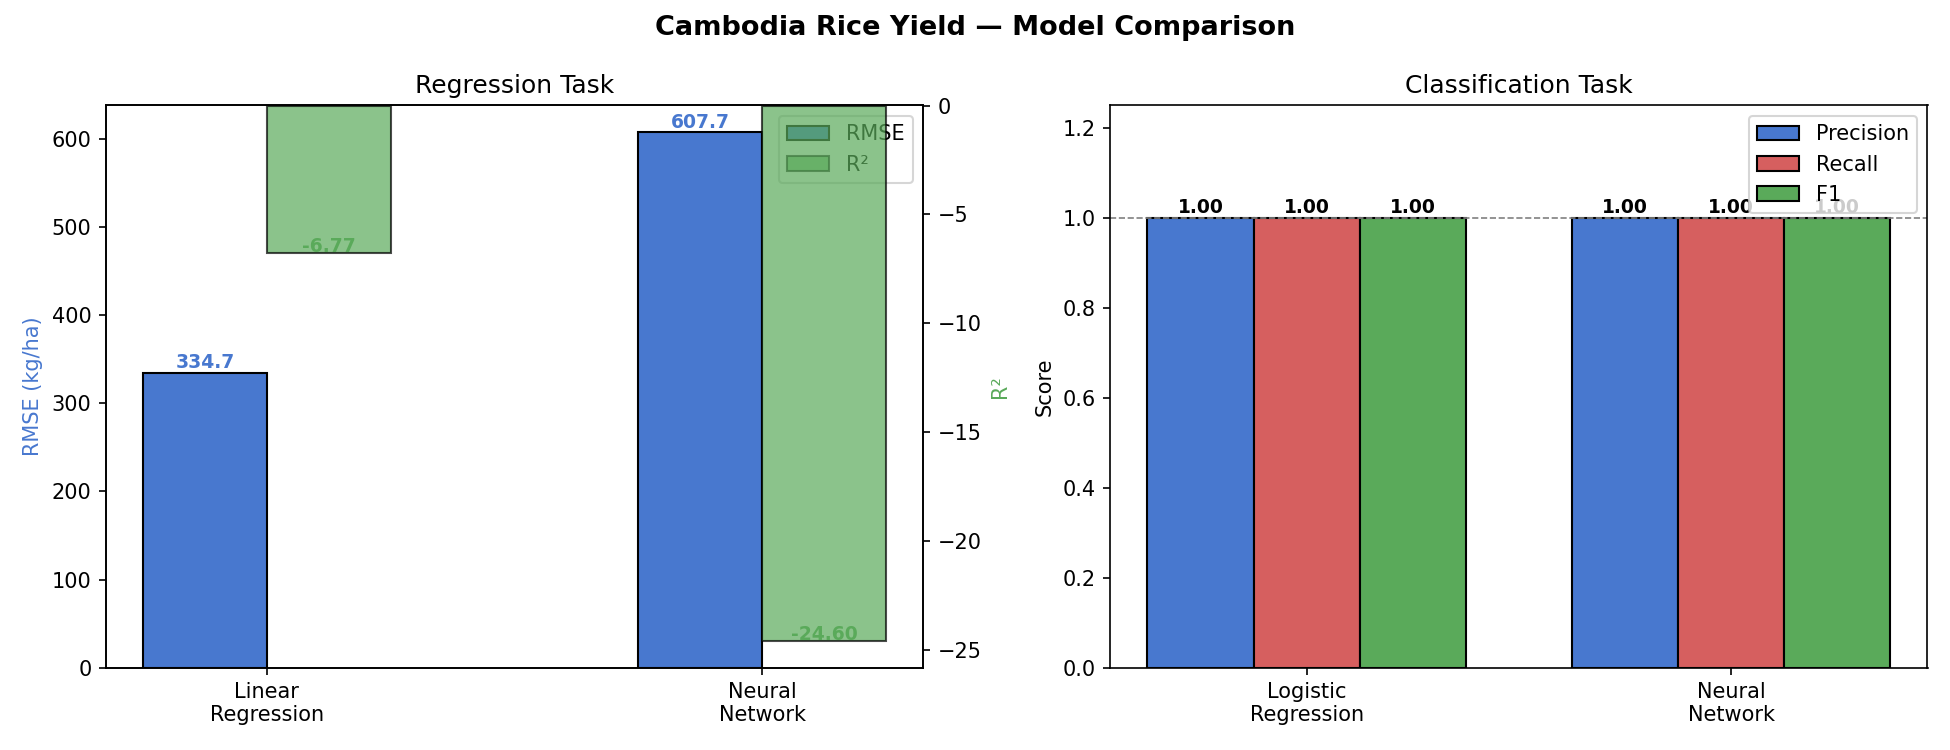
\includegraphics[width=0.92\textwidth]{comparison.png}
    \caption{All models compared on regression (left) and classification (right) tasks.}
  \end{figure}
\end{frame}

% ─────────────────────────────────────────────────────────────────────────────
\section{Conclusion}

\begin{frame}{Conclusion}
  \begin{columns}
    \column{0.55\textwidth}
      \textbf{Key findings:}
      \begin{itemize}
        \item Linear Regression $>$ Neural Network on regression (small data)
        \item Both classifiers achieve perfect F1 due to clean temporal separation
        \item Negative R\textsuperscript{2} highlights the limitation of 35 samples
      \end{itemize}
      \vspace{0.5em}
      \textbf{Future work:}
      \begin{itemize}
        \item Province-level data for larger dataset
        \item Add fertiliser use, flood data, irrigation coverage
        \item LSTM to capture temporal dependencies
      \end{itemize}
    \column{0.45\textwidth}
      \begin{block}{Takeaway}
        For small datasets, simpler models generalise better.
        More data is the most impactful improvement possible.
      \end{block}
  \end{columns}
  \vspace{1em}
  \centering \Large Thank you!
\end{frame}

\end{document}
